\capitulo{5}{Aspectos relevantes del desarrollo del proyecto}

%Este apartado pretende recoger los aspectos más interesantes del desarrollo del proyecto, comentados por los autores del mismo.
%Debe incluir desde la exposición del ciclo de vida utilizado, hasta los detalles de mayor relevancia de las fases de análisis, diseño e implementación.
%Se busca que no sea una mera operación de copiar y pegar diagramas y extractos del código fuente, sino que realmente se justifiquen los caminos de solución que se han tomado, especialmente aquellos que no sean triviales.
%Puede ser el lugar más adecuado para documentar los aspectos más interesantes del diseño y de la implementación, con un mayor hincapié en aspectos tales como el tipo de arquitectura elegido, los índices de las tablas de la base de datos, normalización y desnormalización, distribución en ficheros3, reglas de negocio dentro de las bases de datos (EDVHV GH GDWRV DFWLYDV), aspectos de desarrollo relacionados con el WWW...
%Este apartado, debe convertirse en el resumen de la experiencia práctica del proyecto, y por sí mismo justifica que la memoria se convierta en un documento útil, fuente de referencia para los autores, los tutores y futuros alumnos.


\section{Elección del lenguaje de programación}\label{EleccionLenguaje}

Spark es un sistema que proporciona soporte a diferentes lenguajes de programación: Java, Scala, Python y, recientemente, R~\cite{SparkDoc}. Eliminando este último como posible elección, por el desconocimiento del lenguaje y la poca documentación que hay sobre su uso con Spark, se ha realizado una comparativa entre las opciones restantes para ver cuál de ellas reportaría más ventajas en la realización del proyecto.

Para elegir los aspectos a tener en cuenta durante esta comparación me he basado en el estándar ISO 9126 para la calidad del software~\cite{ISO9126}. Los puntos a analizar han sido finalmente los siguientes: \\

\begin{itemize}
	\item \textbf{Experiencia previa:} Se tendrá en cuenta el contacto que se haya tenido con los lenguajes anteriormente.
	\item \textbf{Eficiencia de ejecución:} Valoraremos el rendimiento de cada lenguaje en función del tiempo que requieren para la ejecución de programas. 
	\item \textbf{Facilidad de mantenimiento:}  Las ventajas y facilidades del lenguaje en el caso de que se requiriese corregir o mantener un algoritmo o aplicación. 
	\item \textbf{Adecuación:} Beneficios aportados por el lenguaje para su uso concreto en el desarrollo de algoritmos para Spark.
	\item \textbf{Documentación disponible:} Facilidad para encontrar información actualizada sobre el uso del lenguaje en Spark.
	
\end{itemize}

Nótese que la tabla \ref{tabla:ComparativaJavaScalaPython} es una comparativa entre las características de los diferentes lenguajes para su uso en Spark, no una comparativa entre las características propias de cada uno a nivel general. Por lo tanto, aspectos que no tengan influencia en Spark o que sean iguales para todos los lenguajes no serán incluidos en la comparativa. Así mismo, si dos lenguajes compartiesen una característica muy parecida o idéntica, esta será incluida una sola vez en la comparativa, fusionando las dos celdas que correspondan.

\tablaApaisadaSmall{Comparativa entre características de Java, Scala y Python para trabajar sobre Spark.}{m{2.65cm} m{5.3cm} m{5.3cm} m{5.3cm}}{ComparativaJavaScalaPython}
{\centering Criterio & \centering Java & \centering Scala  & \multicolumn{1}{c}{Python} \\}{

\centering Experiencia previa & Se ha trabajado en Java múltiples veces durante el grado. & Es un lenguaje sobre el que nunca se ha trabajado. & Se han aprendido las nociones básicas durante la carrera. \\ [0.2cm]


\centering Eficiencia de ejecución & \multicolumn{2}{m{11.05cm}}{Compila los ficheros generando archivos .class y los ejecuta sobre una máquina virtual de Java (JVM). Esto conlleva que la ejecución sea considerablemente más rápida que la del intérprete de Python.} & Es un lenguaje interpretado, lo que afecta negativamente a su rendimiento. Sin embargo, su rendimiento en comparación con Scala mejora considerablemente si contamos con muchos procesadores~\cite{PythonVsScala}.  \\ [0.2cm]


\centering Facilidad de mantenimiento & Código más extenso, aunque la aparición Java 8, con elementos como las funciones lambda han mejorado este aspecto. & \multicolumn{2}{m{11.05cm}}{Menos líneas de código y una sintaxis más fácilmente legible.} \\ [0.2cm]

\centering Adecuación & Trabajar sobre Java nos obliga, a la hora de programar, a transformar estructuras y clases de Spark solo soportadas al trabajar en Scala o Python. Además, no cuenta con un intérprete interactivo. & \multicolumn{2}{m{11.05cm}}{Spark está pensado para trabajar sobre Scala o Python. De hecho, Spark ha sido creado en Scala, por lo que su conocimiento puede ayudar a lo largo del proyecto. Ambos lenguajes cuentan con un intérprete interactivo. } \\ [0.2cm]

\centering Documentación disponible & Existe buena documentación en la página oficial de Spark, aunque es más escasa en otras fuentes. Además, muchas veces la documentación no trabaja sobre Java 8. & \multicolumn{2}{m{11.05cm}}{Existe una amplia documentación sobre el uso de ambos lenguajes en Spark.} \\ [0.2cm]
} 


Como elección final, decidimos que el lenguaje a utilizar será Scala, argumentando lo siguiente sobre los puntos que hemos comparado:

\begin{itemize}
	\item \textbf{Sobre la experiencia previa:} No se considera un problema aprender el lenguaje. Además, los archivos generados tras la compilación y, por consiguiente, la manera de ejecutarlos o monitorizar su rendimiento, es similar a Java, un lenguaje ya conocido.
	\item \textbf{Sobre la eficiencia de ejecución:} El rendimiento, en lo que a tiempo de ejecución se refiere, es muy similar a Java, por lo que se considera una ventaja frente Python.
	\item \textbf{Sobre la facilidad de mantenimiento:} En el momento de la elección del lenguaje no contamos con experiencia en el mantenimiento de un gran código de minería de datos, pero parece lógico que a menos cantidad de líneas que mantener, más fácil puede resultar la tarea.	
	\item \textbf{Sobre la adecuación:} Tras probar Java y Scala con Spark se ha llegado a la conclusión de que el primero implica, no solo más código, sino también operaciones de conversión de estructuras que funcionan en Scala o Python pero son diferentes para Java. Además, frente a Java, Scala cuenta con un intérprete de comandos que nos permite hacer pruebas sin la necesidad de tener que generar y compilar el código cada vez que queramos probar algo.
	\item \textbf{Sobre la documentación disponible:} Scala cuenta, al igual que Python, con una extensa documentación actualizada. Al realizar pruebas con Java en Spark se ha notado un pequeño problema de falta de documentación, pero sobretodo, un problema para encontrar documentación actualizada para aspectos nuevos de Java 8 y que serán frecuentemente usados, concretamente las funciones lambda.
\end{itemize}

\begin{comment}
\newpage
\subsection{Funciones lambda en Java 8 } \label{subsec:ExplLambdaJava}

En Spark, es habitual usar funciones como parámetros de muchas transformaciones y acciones que aplicamos sobre las RDD (ver sección \ref{sec:DefRDD}). Estas funciones, por lo general, son requeridas solamente para la operación concreta, por lo que se suelen definir directamente en el código.

Esto, antes de la llegada de Java 8, generaba un código semejante al siguiente:

\begin{lstlisting}[language=Java,tabsize=4,frame = single,caption=Código de función lambda en Java 7 \cite{Java7vs8},captionpos=b,]
JavaSparkContext sc = new JavaSparkContext()
JavaRDD<String> lines = sc.textFile("hdfs://log.txt")
	.filter(new Function<String, Boolean>() {
		public Boolean call(String s) {
			return s.contains("err");
		}
	});
\end{lstlisting}

Mientras que con Java 8, el código se reduce a:

\begin{lstlisting}[language=Java,tabsize=4,frame = single,caption=Código de función lambda en Java 8 \cite{Java7vs8},captionpos=b,]
JavaSparkContext sc = new JavaSparkContext()
JavaRDD<String> lines = sc.textFile("hdfs://log.txt")
     .filter(s -> s.contains("err"));
\end{lstlisting}

Dado que, como hemos dicho, este tipo de operaciones van a ser enormemente comunes en el desarrollo de algoritmos para Spark, el hecho de poder usar Java 8 puede reducir significativamente el número de líneas de código y, además, facilitar la comprensión del programa.

El uso continuo que se pueden dar a las funciones lambda en la programación con Spark ya se comprobó cuando se intentó programar con Java para Spark.
\end{comment}


\section{Comparativa de rendimiento en la ejecución de clasificaciones entre Weka y Spark}

Como primer aspecto a evaluar durante la realización del proyecto, se llevó a cabo una comparativa entre las ejecuciones que ofrecen Weka y Spark.

La intención de esta prueba era doble: por un lado, suponía un primer acercamiento a la librería Spark y al modelo de funcionamiento en este tipo de entornos. Por otro, se pretendía medir el tiempo de ejecución de Spark frente a alternativas anteriores que, como principal diferencia, no están pensadas para ser ejecutadas en paralelo.

Para realizar las mediciones utilizamos conjuntos de datos de diferentes tamaños, pero siempre un mismo algoritmo: el Naive Bayes. Naive Bayes es un algoritmo de clasificación probabilístico que ya se encontraba implementado tanto en la librería de Weka \cite{John1995} como en la de Spark, razón por la cual ha sido elegido.

Los resultados, así como una explicación más detallada del experimento, pueden encontrarse en el material adjunto a la memoria. Sin embargo, como pequeña aproximación, se muestra en la gráfica \ref{fig:img/compartido/timeTendencyBayes} la evolución del tiempo de ejecución del algoritmo según el número de instancias y según qué configuración de lanzamiento (Weka y Spark con diferente número de ejecutores). Sin entrar a detalle, puede apreciarse claramente una reducción del tiempo de ejecución en Spark a medida que añadimos nuevos ejecutores, lo que se traduce en añadir más unidades de procesamiento a la ejecución. 

	\begin{figure}[!h]
		\centering
		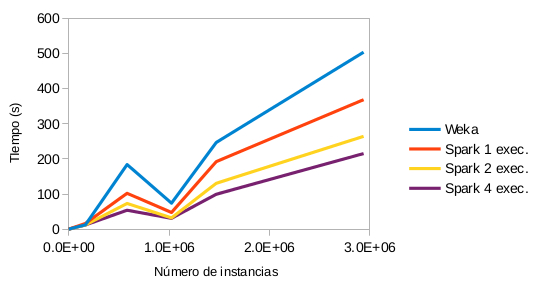
\includegraphics[width=1.0\textwidth]{img/compartido/timeTendencyBayes}
		\caption{Evolución del tiempo de ejecución según el tamaño del conjunto de datos usando Naive Bayes.}\label{fig:img/compartido/timeTendencyBayes}
	\end{figure}

\section{Implementación de algoritmos de selección de instancias}

Marcado como el objetivo fundamental de este proyecto, la realización de dos algoritmos de selección de instancias ha ocupado la mayor parte de tiempo dentro del mismo. A continuación se expondrán algunos de los aspectos que más influencia han tenido durante esta fase de implementación y una pequeña explicación más concreta de la propia implementación de los algoritmos.


\subsection{Indeterminismo, comunicación limitada, grandes conjuntos de datos}

Por la propia naturaleza de la librería, la programación en Spark se ha diferenciado en muchos aspectos del tipo de programación secuencial que se ha aplicado hasta ahora. El hecho de que nuestros algoritmos estén pensados para ejecutarse en paralelo y distribuidos en una gran red de nodos nos proporciona numerosas ventajas, a las que ya nos referimos en las secciones \ref{sec:CompParalela} y \ref{sec:DefEscalabilidad}, pero también plantea problemas que es necesario tener muy en cuenta para la correcta ejecución del programa.

En primer lugar, una ejecución como la nuestra pierde la capacidad de predecir el orden en el que se ejecutarán las operaciones o el propio orden de las instancias cuando son distribuidas o intercambiadas por la red de trabajadores. Este problema ha obligado a modificar el planteamiento inicial de los algoritmos propuestos, pensados para ser ejecutados secuencialmente, y adaptarlos al nuevo escenario.

Así mismo, y con la misma consecuencia, se nos plantea el problema de la comunicación entre nodos. Suponiendo una amplia red de nodos con un gran poder de computación en cada uno de ellos, es sencillo pensar que la comunicación entre ellos puede ser complicada si no queremos que esto afecte de manera muy negativa al rendimiento. Es por ello que Spark no proporciona demasiadas posibilidades en este aspecto o, aquellas que ofrece, son bastante específicas o realmente costosas, como las operaciones de unión (\textit{join}). Todo esto ha sido tenido en cuenta durante la fase de implementación, afectando a las operaciones o incluso a la manera en la que almacenamos los conjuntos de datos, cuyas instancias han sido a menudo ligadas a diferentes valores que permiten controlar el flujo del programa.

Por último, en un intento de optimización por parte de Spark, nos encontramos dentro de la librería la postura de evitar la aparición de operaciones costosas o, por lo menos, realizarlas de manera tal que no tengan un efecto tan perjudicial en el rendimiento. Esto tiene influencia en varios aspectos, siendo el más fácil de entender el de la distribución de las instancias entre los nodos. Algo tan aparentemente sencillo como la división de un conjunto de datos en particiones de igual tamaño, es algo que no ha sido implementado en Spark por el altísimo coste y complejidad que supondría ejecutarlo eficientemente sobre un gran conjunto de datos. En cambio, se proporcionan estrategias basadas en tablas hash o el análisis de pequeños subconjuntos de prueba que permitan realizar la división en particiones aproximadamente iguales. Este tipo de limitaciones han tenido que considerarse cuando hemos necesitado distribuir los nodos de una manera específica.

\subsection{Lazy evaluation}

Un aspecto particular de Spark, y muy importante de cara a la implementación, es el hecho de que Spark utiliza una estrategia de evaluación perezosa (\textit{Lazy Evaluation}), como ya ha sido definido en la sección \ref{sec:DefSpark}.

Esto, si bien se hace en un intento de conseguir optimizar las operaciones, ha de tenerse en cuenta si no se quiere obtener la situación contraria. Hay que comprender que las RDD solo se crean cuando se necesitan y que, por ello, no todas las operaciones se realizan estrictamente en el orden en el que se definen en el código.

En el siguiente ejemplo (\ref{lst:cvScala}), mostramos un fragmento de código que genera un conjunto de pares ``entrenamiento-test'' y realiza sobre cada uno de ellos una operación cualquiera:

\begin{lstlisting}[language=Java,tabsize=4,frame = single,caption=Código de ejecución de una validación cruzada en Scala,captionpos=b,label=lst:cvScala,]

	// Lectura
	val originalData = readDataset(readerArgs)
	// Creación de conjuntos para la validación cruzada
    val cvfolds = createCVFolds(originalData)
    // Por cada conjunto entrenamiento-test
    cvfolds.map {
        case (train, test) => {
          // Realiza operaciones
        }
      }
\end{lstlisting}

Una primera impresión del código \ref{lst:cvScala} puede hacernos suponer que primero se generan todos los subconjuntos y, posteriormente, sobre cada uno de ellos se realiza la operación que se le pide. Sin embargo, el comportamiento real es muy distinto y es que, hasta que no necesitamos los conjuntos ``train'' y ``test'' dentro del bucle, no calculamos dichos conjuntos. De esta manera, cada vez que realicemos una iteración del bucle calcularemos solo los conjuntos que vayamos a necesitar para esa iteración.

Tener esto en cuenta es importante a la hora de programar, pues puede provocar, entre otros aspectos negativos, cuellos de botella, excesivo uso de almacenamiento con datos que no van a usarse en un futuro cercano o necesidad de recalcular grandes estructuras RDD.

\subsection{Correcta gestión de los recursos}

Como se ha mencionado anteriormente en esta memoria (ver sección \ref{sec:DefSpark}), una de las ventajas de Spark frente a otras alternativas es, no solo la posibilidad de usar diferentes niveles de almacenamiento, sino también la posibilidad de definir nosotros qué almacenar y dónde hacerlo.

Aunque parezca un aspecto con importancia menor, solo útil cuando se busca optimizar al máximo una operación, lo cierto es que es un aspecto sumamente importante que tiene una altísima influencia en el tiempo de ejecución. Tener en mente qué estructuras RDD almacenar, dónde hacerlo o si realmente merece la pena ocupar espacio ante una operación que podría recalcularse es algo que se ha visto completamente necesario desarrollando el proyecto.

Tomemos como ejemplo el algoritmo DemoIS, donde se decidió persistir una estructura RDD generada tras la fase de votaciones. Podemos ver como el tiempo de ejecución de algunas de las operaciones ha sido reducido del orden de segundos (en la imagen \ref{fig:img/memoria/DemoISWithoutPersist}) al tiempo de milisegundos (en la imagen \ref{fig:img/memoria/DemoISWithPersist}).

	\begin{figure}[!h]
		\centering
		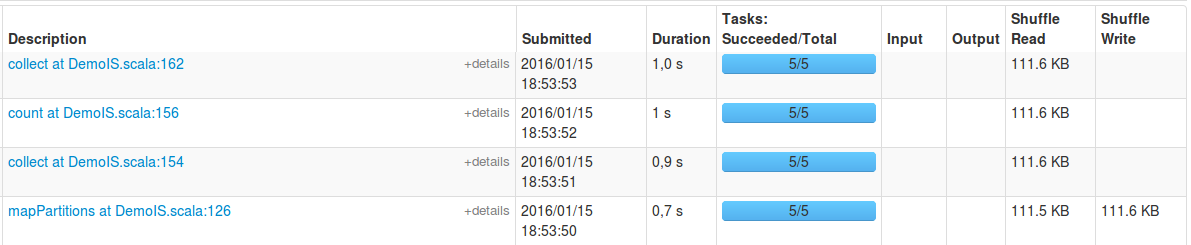
\includegraphics[width=1.0\textwidth]{img/memoria/DemoISWithoutPersist}
		\caption{Ejecución de operaciones en el algoritmo DemoIS sin persistir ninguna RDD.}\label{fig:img/memoria/DemoISWithoutPersist}
	\end{figure}
	\FloatBarrier
	
		\begin{figure}[!h]
		\centering
		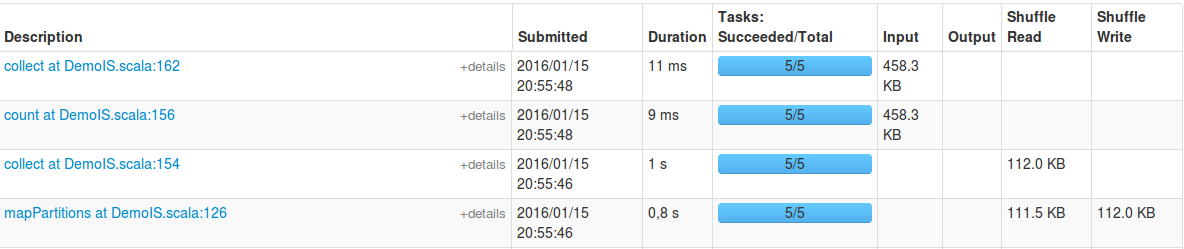
\includegraphics[width=1.0\textwidth]{img/memoria/DemoISWithPersist}
		\caption{Ejecución de operaciones en el algoritmo DemoIS persistiendo el conjunto de datos tras las votaciones.}\label{fig:img/memoria/DemoISWithPersist}
	\end{figure}
	\FloatBarrier


Así mismo, también es necesario tener en cuenta la manera en la que se realizan las operaciones. Un punto importante de Spark es que necesita escribir los datos a disco cuando quiere redistribuirlos por la red de nodos, por si necesitase recuperarse de algún fallo. Escribir a disco es una operación muy costosa, por lo que se ha de intentar reducir al mínimo. El orden de las operaciones o el uso de diferentes operaciones para llegar a un mismo resultado, han sido considerados para aumentar el rendimiento de nuestro programa.

Un ejemplo lo encontramos entre el uso de dos funciones que las RDD proporcionan: \textit{reduceByKey} y \textit{groupByKey}. Aunque a menudo los resultados alcanzados por una de las funciones puede ser conseguido mediante la otra, \textit{groupByKey} obliga a escribir a disco la estructura RDD completa, mientras que \textit{reduceByKey} reduce considerablemente esta operación \cite{ShuffleSpark}. Problemas similares ocurren con funciones como los \textit{join} o \textit{subtractByKey}, utilizada también en este proyecto.

\subsection{Implementación de resursos necesarios}\label{sec:ImplRecursosAdicionales}

Como ya se ha comentado anteriormente, la librería MLlib de Spark con la que hemos estado trabajando aún se encuentra en una fase donde no contamos con una amplia colección de clases. Es por ello que han tenido que implementarse algunos algoritmos adicionales a los propuestos como objetivo. Cabe destacar:

\begin{itemize}
\item \textbf{Algoritmo Condensed Nearest Neighbour (CNN):} Un algoritmo de selección de instancias simple y cuya ejecución es secuencial. Ha sido incluido de manera obligatoria para poder ejecutar correctamente nuestro algoritmo Democratic instance selection (ver algoritmo en la sección~\ref{sec:defDemoIS}).
\item  \textbf{Algoritmo \textit{k}-Nearest Neighbours (\textit{k}NN):} Un clasificador simple, necesario tanto para la implementación de Democratic instance selection como para comparar el funcionamiento de nuestros selectores de instancias. Está programado de manera secuencial, de manera que requiere que todos los datos sean recogidos en una sola máquina para poder aplicar el algoritmo. En un primer momento se creyó que podríamos contar con una implementación en Spark del \textit{k}NN gracias al material presentado en la Conferencia de la Asociación Española para la Inteligencia Artificial 2015 (CAEPIA 2015) \cite{KNNConferencia}, pero finalmente tuvo que implementarse una versión menos ambiciosa del clasificador.
\end{itemize}


\subsection{Implementación concreta de LSHIS}

Dadas las restricciones ya mencionadas en esta misma sección, la implementación del algoritmo LSHIS ha sufrido modificaciones con respecto a su propuesta original, cuyo pseudocódigo puede verse en el algoritmo \ref{alg:LSHIS}.

Podemos ver una nueva versión del método en el pseudocódigo \ref{alg:LSHISSPARK}. El cambio fundamental puede apreciarse cuando existen dos o más familias de funciones hash. Por culpa del indeterminismo que genera la ejecución en paralelo nos vemos obligados a ejecutar una serie de operaciones sobre conjuntos que no eran necesarias en la ejecución secuencial, donde se solucionaba el problema mediante el uso de un nuevo bucle \textit{for}.

Cabe destacar que estas operaciones realizadas cuando hay dos o más familias de funciones hash no usan en ningún momento el conjunto de instancias completo, sino que usan el conjunto solución generado por iteraciones anteriores y el conjunto solución generado por esta nueva iteración, ambos suponiéndose más pequeños que el conjunto inicial. Esta es una consideración muy importante en comparación con otras alternativas que surgieron, porque implica que la carga de trabajo va a ser menor que si tuviésemos que operar con todo el conjunto de instancias inicial.

%IMPLEMENTACIÓN ACTUAL LSHIS

%LSH_IS_S
\begin{algorithm*}
\DontPrintSemicolon
\KwIn{Conjunto de instancias $ X = \lbrace(\mathbf{x}_{1},y_{1}),...,(\mathbf{x}_{n},y_{n})\rbrace$,
      conjunto $\mathcal{G}$ de familias de funciones hash}
\KwOut{Conjunto de instancias seleccionado $ S \subset X $ }

$ S = \varnothing $

\ForEach {familia de funciones hash en $\mathcal{G}$} {

  \ForEach {instancia $\mathbf{x}$ en $X$} {
        $\{u,c\}\leftarrow$ tupla formada por la cubeta asignada a $\mathbf{x}$ y su clase

        Asociar $\mathbf{x}$ a su tupla $\{u,c\}$
    }

    $sel\leftarrow$ Seleccionar una instancia aleatoria por cada par llave $\{u,c\}$

    \If {es la primera iteración}{
    $ S = sel $
    }
    \Else{

    \ForEach {instancia $\mathbf{x}$ en S} {
            $\{u,c\}\leftarrow$ tupla formada por la cubeta asignada a $\mathbf{x}$ y su clase

    Asociar $\mathbf{x}$ a su tupla $\{u,c\}$

    }

    Añadir a $S$ aquellas instancias de $sel$ que no seleccionadas en $S$
    }

}

\Return {$S$}
\caption{LSH-IS -- Implementación paralela en Spark}
\label{alg:LSHISSPARK}
\end{algorithm*}

Como del pseudocódigo anterior no puede deducirse con claridad cómo están estructuradas las operaciones dentro del entorno paralelo, se incluyen los siguientes diagramas (ver imágenes \ref{fig:img/memoria/diagram_LSHIS1} y \ref{fig:img/memoria/diagram_LSHIS2}) que permiten identificar como se realizan las operaciones dentro de un grupo de nodos. Compruébese que todas las operaciones se ejecutan en paralelo. Los bloques de ``Conjunto de datos inicial'' y ``Solución'' simplemente han sido añadidos para aclarar el diagrama, pero tanto los datos iniciales como el resultado podrían perfectamente ser datos que ya se encontrasen distribuidos.

	\begin{figure}[!h]
		\centering
		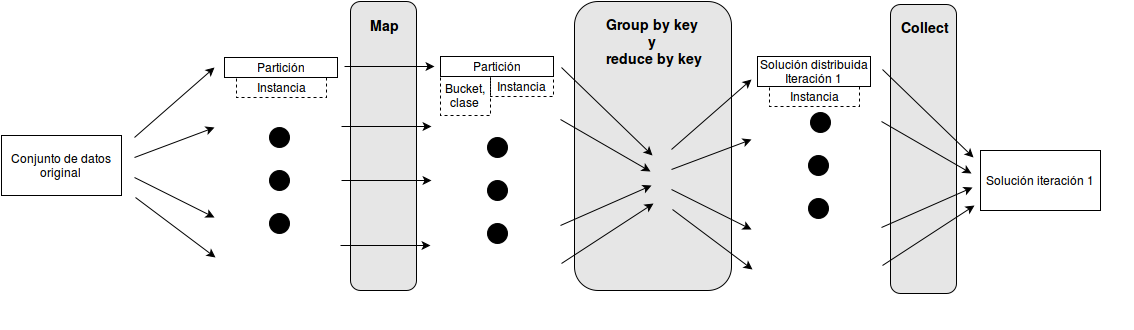
\includegraphics[width=1.0\textwidth]{img/memoria/diagram_LSHIS1}
		\caption{Diagrama de la ejecución del algoritmo LSHIS durante su primera iteración.}\label{fig:img/memoria/diagram_LSHIS1}
	\end{figure}
	\FloatBarrier
	
		\begin{figure}[!h]
		\centering
		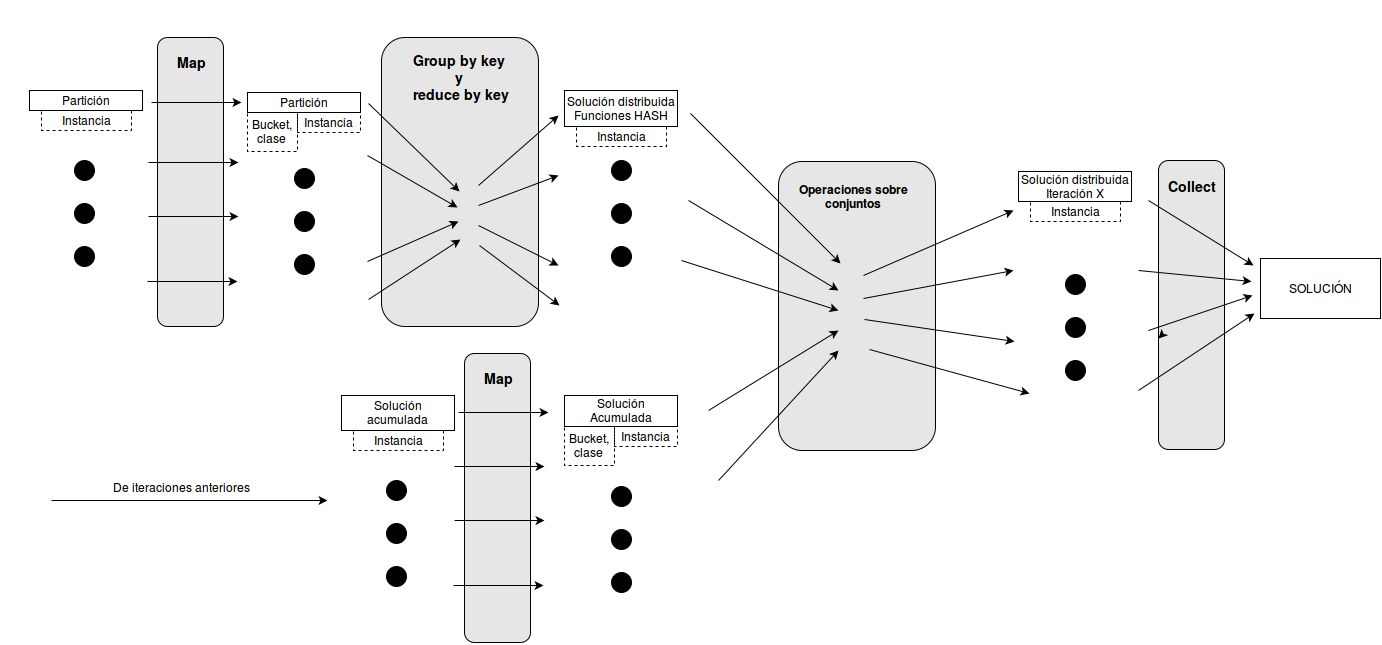
\includegraphics[width=1.0\textwidth]{img/memoria/diagram_LSHIS2}
		\caption{Diagrama de la ejecución del algoritmo LSHIS durante su segunda iteración y sucesivas.}\label{fig:img/memoria/diagram_LSHIS2}
	\end{figure}
	\FloatBarrier

%\imagen{img/memoria/diagram_LSHIS1}{Diagrama de la ejecución del algoritmo LSHIS durante su primera iteración.}
%\imagen{img/memoria/diagram_LSHIS2}{Diagrama de la ejecución del algoritmo LSHIS durante su segunda o mayor iteración.}


\subsection{Implementación concreta de DemoIS}

La implementación de este algoritmo no ha requerido modificar el pseudocódigo del mismo, que puede verse en la sección \ref{sec:defDemoIS}). Sin embargo, sí existen varios detalles que conviene destacar sobre la actual implementación.

En primer lugar, como puede apreciarse en la figura \ref{fig:img/memoria/diagram_DemoIS}, no todo el algoritmo se ejecuta en paralelo. A la hora de calcular el \textit{fitness} óptimo lo hacemos de manera secuencial. Esto es así porque no contamos con una implementación paralela del algoritmo \textit{k}NN, necesario para este proceso. Aún con esto, durante esa etapa del proceso solo seleccionamos un pequeño grupo de instancias en comparación con el conjunto inicial, por lo que operar con tal número de datos no supone un problema de rendimiento tan grande.

Existen otras consideraciones de cara a la implementación, como el uso de un particionador aleatorio que no genera particiones del mismo tamaño, por lo mencionado anteriormente, o la creación de una clase individual que evite la serialización completa del algoritmo al realizar la primera operación \textit{map}. Esto último, será tratado con más detenimiento en el anexo de diseño incluido junto con la memoria.

%En segundo lugar, el particionado del conjunto de datos inicial para realizar las votaciones es aleatorio y genera particiones que no son estrictamente del mismo tamaño, sino que presentan ligeras variaciones de unas a otras. Esto es así porque, en un entorno paralelo, es muy complicado redistribuir las instancias entre los nodos de manera aleatoria pero, a la vez, generando particiones de tamaño similar (y, es por ello, que Spark no proporciona ningún tipo de clase o ayuda en este aspecto). Dado que estos algoritmos están pensados para su ejecución con un número muy grande de instancias, se confía en que la aleatoriedad sitúe un número muy similar de instancias en cada una de las particiones.

	\begin{figure}[!h]
		\centering
		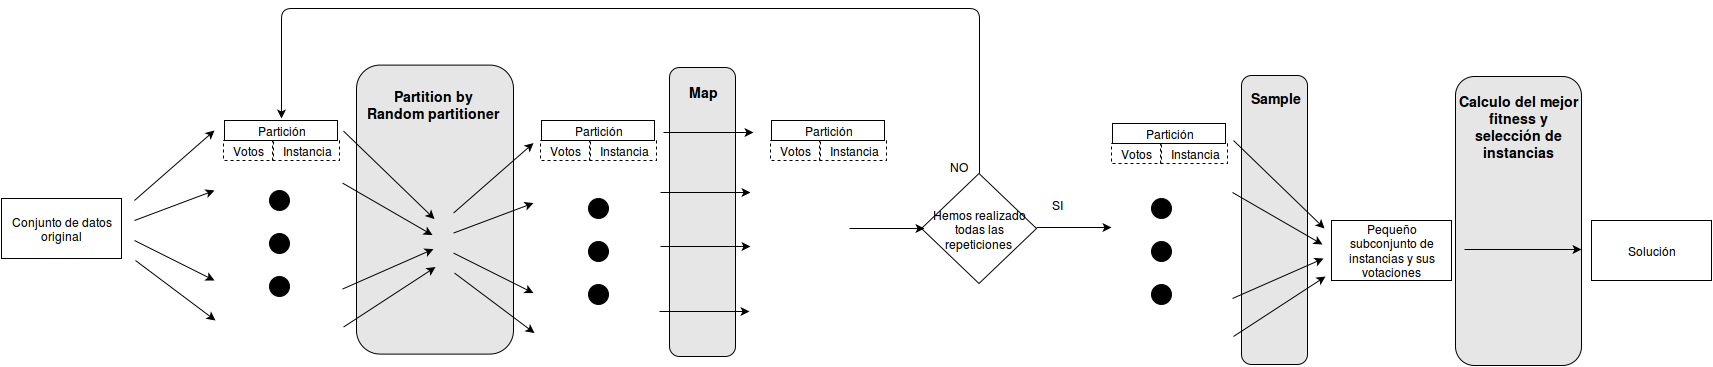
\includegraphics[width=1.0\textwidth]{img/memoria/diagram_DemoIS}
		\caption{Diagrama de la ejecución del algoritmo DemoIS.}\label{fig:img/memoria/diagram_DemoIS}
	\end{figure}
	\FloatBarrier

%\imagen{img/memoria/diagram_DemoIS}{Diagrama de la ejecución del algoritmo DemoIS.}

\section{Comparativa entre las implementaciones de Weka y Spark}

Como otro de los objetivos principales del proyecto, se procedió a realizar una comparación entre nuestras implementaciones de los algoritmos de selección de instancias con las ya existentes para su uso en Weka.

De nuevo, la finalidad de esta comparación tenía varios objetivos: evaluar el rendimiento entre ambas aproximaciones, comprobar el correcto funcionamiento de los algoritmos y evaluar como los cambios de implementación podían haber afectado a su funcionalidad.

Aunque se proporciona más información en los documentos anexos, podemos observar en las gráficas \ref{fig:img/compartido/timeTendencyLSH4} y \ref{fig:img/compartido/timeTendencyLSH4} una evolución del tiempo de ejecución según el algoritmo y la cantidad de datos analizados. Para ello se proporcionan varios tipos de ejecuciones, pudiéndose diferenciar uno para Weka y otros para Spark con diferente número de ejecutores.

Puede verse claramente que, pese a su ejecución en paralelo, el algoritmo LSHIS continúa siendo más rápido en su ejecución secuencial. Esto es debido en parte a que es un algoritmo muy rápido incluso cuando se aplica sobre un número de instancias grande. Por otro lado, DemoIS proporciona, desde un primer momento y con un conjunto de datos relativamente pequeño, mejores tiempos que la implementación anterior.

	\begin{figure}[!h]
		\centering
		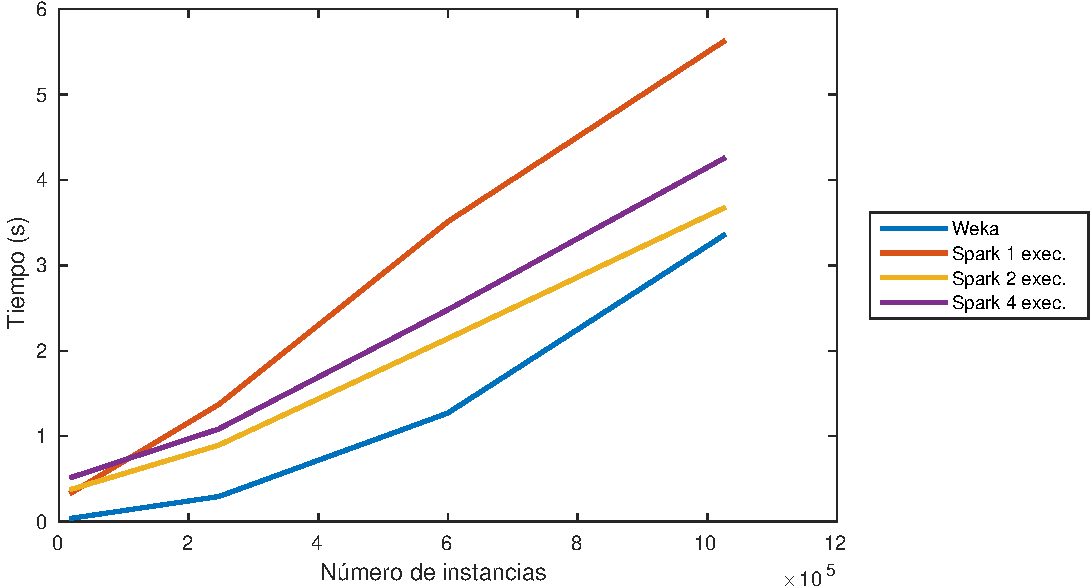
\includegraphics[width=1.0\textwidth]{img/compartido/timeTendencyLSH4}
		\caption{Evolución del tiempo de ejecución según el tamaño del conjunto de datos usando LSHIS.}\label{fig:img/compartido/timeTendencyLSH4}
	\end{figure}
	
		\begin{figure}[!h]
		\centering
		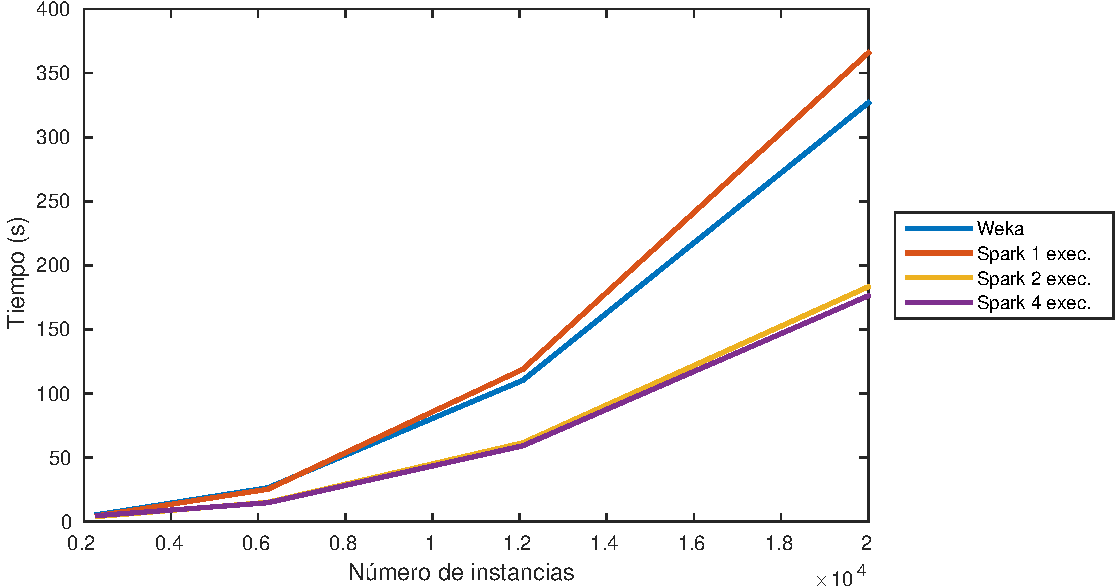
\includegraphics[width=1.0\textwidth]{img/compartido/timeTendencyDIS4}
		\caption{Evolución del tiempo de ejecución según el tamaño del conjunto de datos usando DemoIS.}\label{fig:img/compartido/timeTendencyDIS4}
	\end{figure}
	\FloatBarrier


\section{Ejecución en la nube}\label{sec: ejecucionNube}

Una vez se comprobó el buen funcionamiento del proyecto, se procedió a desplegar el trabajo en el entorno en el que está destinado a ser ejecutado: un clúster real.

Este despliegue se ha realizado en dos plataformas diferentes:
\begin{itemize}
	\item Google Cloud Dataproc \cite{dataprocSoft}: Servicio, actualmente en estado \textit{beta}, que Google ofrece para lanzar tareas de minería de datos en un clúster propiedad de la compañía. Utilizando una versión de prueba, los recursos han sido limitados (máximo de 8 procesadores por cluster), pero eso no ha impedido realizar lanzamientos correctamente.  
	\item Servidor Clúster Dell: Un servicio al que la Universidad de Burgos tenía acceso y en el cual se ha permitido lanzar algunas ejecuciones. Este clúster está configurado con un sistema de colas de trabajo PBS (\textit{Portable Batch System}), por lo que se ha necesitado de un script propuesto por la Universidad de Ohio \cite{baer2015integrating} para ejecutar nuestras pruebas. Aunque se han tomado algunas mediciones sobre el comportamiento de nuestra aplicación en este entorno, se han encontrado dificultades al lanzar Spark sobre este tipo de sistema de gestión, donde algunos nodos quedaban bloqueados durante la ejecución presumiblemente por la falta de recursos.
\end{itemize}

Por las características de los servicios en los que se ha desplegado el programa, se necesitó realizar pequeños cambios en la implementación y definir una versión anterior de Scala a la hora de compilar el código.

Puede encontrarse información más concreta sobre cómo realizar experimentos sobre Google Cloud Dataproc en el manual del usuario anexo a esta memoria. Igualmente, resultados sobre las pruebas realizadas en estos servicios o pequeñas consideraciones a tener en cuenta en la etapa de implementación pueden encontrarse en los documentos ``Pruebas del sistema'' y ``Manual del programador'' respectivamente. 

\section{Implementación de un entorno gráfico}

En la etapa final, se vio como el proyecto había alcanzado una complejidad considerable en cuando a las opciones de lanzamiento se refiere. Este hecho hacía de la ejecución por línea de comandos un método de lanzamiento mucho más tedioso de lo que a un usuario normal podría resultarle ya de principio. Es por esta razón que, con la intención de facilitar el uso de la biblioteca, se decidió la implementación de una pequeña interfaz gráfica que hiciese más intuitivo el uso del proyecto.

Así pues, se ha realizado una interfaz gráfica que permite introducir, mediante campos de texto, todas las opciones necesarias para la ejecución de los algoritmos. Además, posibilita la acción de crear baterías de ejecuciones al dar la opción de indicar más de una configuración de Spark, conjunto de datos y/o filtro a la vez.

Esta interfaz ofrece dos modos de ejecución:

\begin{itemize}
\item Permite ejecutar los algoritmos directamente desde la interfaz gráfica. Es una opción no recomendada si lo que se busca es eficiencia en los tiempos de ejecución pero es una manera sencilla de realizar pruebas en modo local.
\item Permite la compresión, en un archivo de extensión .zip, de todos los conjuntos de datos necesarios para lanzar las ejecuciones definidas. Además, también proporciona un script .sh para realizar las ejecuciones indicadas. Este tipo de operación facilita que el usuario pueda definir todas las operaciones desde su máquina y, posteriormente, pueda trasladarlas de manera sencilla a un servidor más potente donde serán ejecutadas.
\end{itemize}

Después de la creación y revisión de algunos prototipos no funcionales, la apariencia final del producto evolucionó hasta alcanzar el aspecto que muestra la figura \ref{fig:img/memoria/full_interface}.

\imagen{img/memoria/full_interface}{Apariencia final de la interfaz gráfica del proyecto.}

